\documentclass[UTF8]{ctexart}

\usepackage{subfiles}  

%下面的语句, 引入你的头部设置文件
\usepackage{C:/phpStorm_proj/02_myself_ID_EGO/+100_latex_all_math_sel/myPreamble} 
%必须是绝对路径,才能让各个tex在单独编译时使用到

\title{积分}


%---------------------------------


\begin{document}
	\tableofcontents % 生成目录
	\date{} % 若不写这句, 则默认也会渲染出日期, 所以我们要手动赋空值
	\maketitle  %这行代码, 让你前面的 title, author, date生效
	
	\part{积分 integral}
	
	对于曲线f 下的面积, 如果我们能找到一个函数I 来表示它, 那么这个函数I, 就叫做f的``积分".
	
	积分很有用, 是因为很多生活中实际的问题, 都能近似成``大量很小的东西加起来". 而这样的问题都能转化成求某图像下的面积. 所以, 我们要找的, 就是这个能表示面积的"积分函数".
	
	
	
	
	
	
	\part{不定积分 indefinite integral : 即``原函数"}
	
	一个原函数, 求其导数, 能得到"导函数". \textbf{反过来, 从``导函数"算出其``原函数"的过程, 就是求其``不定积分". 换言之, ``原函数"的别名就是"不定积分".}
	
	如: ``原函数"是 F(x), 其``导函数"是 D(x), 即: $ F'(x) = D(x)$, 则  原函数 F(x) 就是 D(x) 的其中一个原函数. \\
	
	为什么是``其中一个"原函数? 因为可以有无穷多个原函数, 它们都能得到同一个导函数. 比如, 这些原函数: $x^2,  x^2+3$, 它们都能得到同一个导函数 $2x$.
	
	其规律就是: $\left( \underset{\text{原函数}}{\underbrace{F\left( x \right) }}+\underset{\text{常数}}{\underbrace{C}} \right) '=\underset{\text{导函数}}{\underbrace{D\left( x \right) }} $ \\
	\\
	
	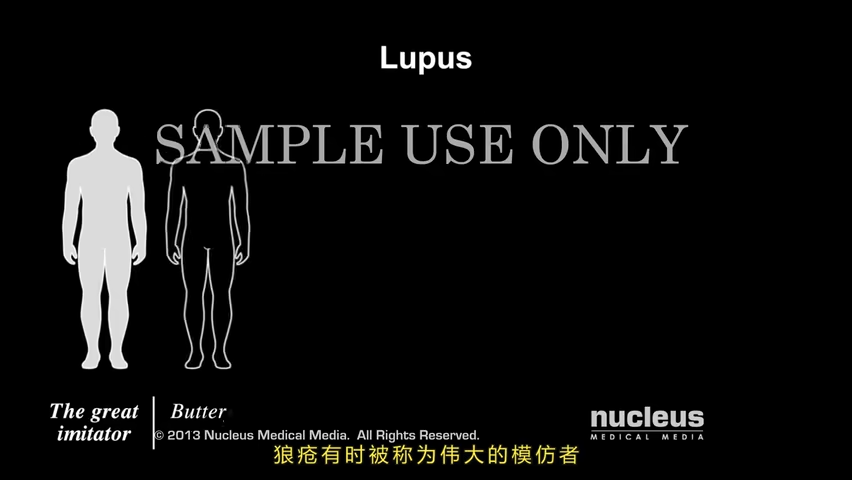
\includegraphics[width=0.3\textwidth]{/0055.png} \\
	
	所以, 从``导函数"来反求其``原函数", 就是求``不定积分". 因此, ``原函数"的别名就是``不定积分".
	
	即: $\int_{}^{}{\underset{\text{导函数}}{\underbrace{D\left( x \right) }}dx=\underset{\text{原函数}}{\underbrace{F\left( x \right) }}+\underset{\text{常数}}{\underbrace{C}}} $ \\
	
	
	符号 $\int$ 是英文 sum 的 首字母s 变形. \\
	
	
	
	Σ 和 $\int$ 的区别: 
	
	\begin{tabular}{|l| l| }
		\hline
		Σ &  通常是对``有限个", 或者``离散的量"求和。 \\
		\hline
		$\int$ & 是对``无穷个"连续的``无穷小量"的求和 \\
		\hline
	\end{tabular} \\

	类似的:
	
	\begin{tabular}{|l| l| }
		\hline
		Δ & 表示``有限小"的变量. \\
		\hline
		dx & 表示``无穷小"变量. 有 x →0 这个``极限"的概念在里面. \\
		\hline
	\end{tabular}





	


	
	
	
	
	
	
	
	
		
	
\end{document}


